
\begin{table}[t!]
\resizebox{8cm}{!} {
\centering

    \begin{tabular}{|lllll|}
    \hline
    \textbf{Category}  &  \textbf{No. of }   & \textbf{Avg. No. of }   &  \textbf{Avg. Doc. }	&  \textbf{Avg. Person }	\\  
    & \textbf{People} & \textbf{Documents} & \textbf{Length} &  \textbf{Name } \\
    & & & & \textbf{Frequency} \\  \hline
Not Influ. & 36004 & 1.04 & 2119.6 & 1.07 	\\ \hline
 Popular & 344 & 5.75 & 1976.3 & 6.68  \\ \hline
Elite & 16 & 22.8 & 2971.5 & 29.870	 \\	\hline 
  \end{tabular}}
\caption {Table illustrating average statistics for each Person Category of the People Gazetteer.}
\label{table:stats}  
%\vspace*{-10pt}
\end{table}

We present statistics pertaining to each category (not influential, popular and elite) of the people gazetteer in Table~\ref{table:stats}. 
It is observed that, on average the \emph{elite} are discussed very often in the news articles.
Document Length need not be high for a person to be more influential -- average document length obtained for the popular group is high in spite of their average IPI being low. This indicates that the number of similar articles for each document as well as the person name frequency play an important part in measuring influence.\\
\noindent \textbf{Effect of varying the number of topics in the topic model: } Our objective is to study the sensitivity of the ranked lists to parameters of the ADIP algorithm. We study the effect of the number of topics used in the LDA Model on the influential people list.
Two ranked lists of influential people, $L_1$ and $L_2$ are compared by using 30 and 100 topics\footnote{Several topic models are built by varying parameters of AD-LDA algorithm including number of iterations, topics and processors and their \emph{perplexity} is measured. Models with less perplexity are used for the study.} respectively. The weights $w_a$, $w_b$ and $w_c$ are set to 1 to ensure that all parameters have equal importance during calculation of DI and IPI. Figure~\ref{figure:IPI} shows the average IPI from the two ranked lists -- it appears that the average IPI for highly influential people is more susceptible to changes in number of topics.

%The statistics obtained from both lists with respect to each person category of the people gazetteer are shown in Table~\ref{table:stats}. 
%It can be clearly observed from the table that Highly Influential Persons occur in most number of news articles on an average and with highest average term frequency followed by Medium Influential and Marginal Influential Persons.
%Document Length need not always be too high for a person to be ranked higher as can be observed from the fact that average document length obtained for Marginally Influential People is high in spite of their Average IPI being low indicating that the varying number of similar articles for each document as well as its Term Frequency share also play an important part in measuring influence. 
%The following sections present comparison between the ranked influential person lists L1 and L2, some case studies and evaluation results:
 
\begin{table*}
\centering

\resizebox{15cm}{!}{
\begin{tabular}{|p{2cm}|l|p{1.5cm}|p{1.5cm}|l|l|l|p{3cm}|l|l|}
\hline
Person Name    & IPI  & Number of Articles & Person Category & NDL  & NPNF  & NSIM & TOPIC WORDS                                                          & UniqT & Rank \\ \hline
capt creeten   & 3.32 & 10                 & Popular          & 0.55 & 1.9 & 0.8  & mr court police judge justice case yesterday street district         & 0.06  & 1    \\ \hline
capt hankey    & 3.05 & 5                  & Popular          & 0.68 & 1.69  & 0.6 & club game team play football half ball left college back             & 0.06  & 2    \\ \hline
capt pinckney  & 2.93 & 3                  & Not Inf.        & 0.38 & 1.84 & 0.67 & man ho men night back wa room left house told bad                    & 0.03  & 3    \\ \hline
john martin    & 2.89 & 14                 & Popular          & 0.55 & 1.6  & 0.57  & mr court police judge justice case yesterday street district witness & 0.16  & 4    \\ \hline
ann arbor   & 2.87 & 44		    & Elite		& 0.19   & 1.77     & 0.63    &  dr book st story books cloth author cure free work york blood   illustrated remedy goods medical library health price & 0.26 & 5	\\  \hline
john macdonald & 2.85 & 3                  & Not Inf.        & 0.55 & 2.2  & 0    & great people life man women good country world american part         & 0.1   & 6    \\ \hline
aaron trow     & 2.81 & 1                  & Not Inf.        & 0.7  & 2.07 & 0    & man ho men night back wa room left house told                        & 0.03  & 6    \\ \hline
mrs oakes      & 2.79 & 5                  & Popular          & 0.08 & 2.04 & 0.6  & street mrs mr avenue wife house miss yesterday years home            & 0.06  & 7    \\ \hline
alexander iii  & 2.71 & 31                 & Elite            & 0.24 & 2.04 & 0.25 & great people life man women good country world american part         & 0.16  & 9    \\ \hline
buenos ayres   & 2.7 & 6                  & Popular          & 0.49 & 1.47  & 0.67 & white water indian black long found thu big dog time                 & 0.06  & 10    \\ \hline
\end{tabular}}
\caption{Table showing top 10 influential persons of List L1 detected from People Gazetteer with 30 Topics LDA model. Parameters NDL, NPNF, NSIM and Topic Words belong to the maximum scoring DI in the person's document list.}
\label{table:30t}
%\vspace*{-10pt}

\end{table*}


\begin{table*}
\centering
\resizebox{15cm}{!} {
\begin{tabular}{|p{2cm}|l|p{1.5cm}|p{1.5cm}|l|l|l|p{3cm}|l|l|}
\hline
Person Name    & IPI  & Number of Articles & Person Category        & NDL  & NPNF  & NSIM & Topic Words                                                                 & UniqT & Rank \\ \hline
capt creeten   & 3.28 & 10                 & Popular     & 0.55 & 1.90 & 0.8  & mr police witness committee capt asked captain money inspector paid         & 0.06  & 1    \\ \hline
mrs martin     & 3.21 & 8                  & Popular     & 0.20 & 2.36 & 0.62  & mrs mr years wife home house ago woman city died                            & 0.02  & 2    \\ \hline
capt hankey    & 2.97 & 6                  & Popular    & 0.68 & 1.69  & 0.8 & game team football play half line ball back yale eleven                     & 0.02  & 3   \\ \hline
alexander iii  & 3.05 & 31                 & Elite     & 0.49 & 2.04 & 0.45 & emperor prince french alexander czar london nov government imperial russian & 0.07  & 4    \\ \hline
aaron trow     & 2.79 & 1                  & Not Inf. & 0.70 & 2.07 & 0    & day place long great water time feet found good men                         & 0.01  & 5    \\ \hline
john martin    & 2.78 & 14                 & Popular     & 0.55 & 1.6  & 0.57  & mr police witness committee capt asked captain money inspector paid         & 0.05  & 6    \\ \hline
john macdonald & 2.77 & 3                  & Not Inf. & 0.55 & 2.2  & 0    & people american man great country men world life good english               & 0.02  & 7    \\ \hline
mrs oakes      & 2.74 & 5                  & Popular     & 0.08 & 2.04 & 0.6  & mrs mr years wife home house ago woman city died                            & 0.02  & 7    \\ \hline
ed kearney     & 2.63 & 7                  & Popular     & 0.16 & 1.6  & 0.85 & won time race ran mile furlough half lo track fourth                        & 0.01  & 9    \\ \hline
caleb morton   & 2.61 & 1                  & Not Inf. & 0.70 & 1.9  & 0    & day place long great water time feet found good men                         & 0.01  & 10   \\ \hline

\end{tabular}}
\caption{Table showing top 10 influential persons of  List L2 detected from People Gazetteer with 100 Topics LDA model. Parameters NDL, NPNF, NSIM and Topic Words belong to the maximum scoring DI in the person's document list.}
\label{table:100t}
\vspace*{-10pt}
\end{table*}

%\subsection{Comparison Across Ranked Influential Person Lists }

The top 10 influential people from lists $L_1$ and $L_2$ are presented in Tables~\ref{table:30t} and ~\ref{table:100t} respectively. 
%It can be clearly seen from both the tables that the person category labels assigned during development of people gazetteer do not hold true after detection of influential persons. This suggests that the highly influential category people which were defined as person entities with more than 16 articles in the dataset might not necessarily be the most influential. The top 10 influential persons in both tables are dominated by the not influential and popular category having considerably less number of articles of occurrence. This indicates that the number of articles  has not been given priority while measuring influence. 
Our results suggest that none of the measures of NDL, NPNF or NSIM can be used alone to say whether a person is influential since these value do not decrease or increase consistently although the NPNF measure does contribute most to the IPI of any person.

%\newpage
The ranked lists $L_1$ and $L_2$ can be compared in terms of NSIM, UniqT and topic words to see the effect of 30 and 100 topics LDA models on influential person detection.
 If NSIM remains same in $L_1$ and $L_2$ during influential person detection, then the same highest scoring article DI is selected for calculation of IPI in both of them. This is why the parameters NDL and NPNF remain same across both the lists. This can be seen for ``capt creeten", ``capt hankey", ``aaron trow" and ``mrs oakes" in Tables~\ref{table:30t} and ~\ref{table:100t}. However, the value of UniqT for these persons decreases leading to decrease in their final IPI. This is because if the LDA model with higher number of topics (100) is used, the proportion of unique topics becomes lower when NSIM does not change. When the NSIM value changes because of change in number of topics, a different article with maximum DI score can get selected leading to change in the values of NDL, NPNF, UniqT and the final IPI. This causes a shift in the ranking of influential persons across the two lists and can be seen when the rank of ``alexander iii" in the first table moves from 9 to 4 in the second table. 
This helps to illustrate how a change in number of topics affects the ranking of influential people.

Wilcoxon signed rank paired test is also performed on the ranks of influential people across the two lists $L_1$ and $L_2$. This is done to test the hypothesis whether the differences in the ranking of person entities obtained using the 30 topic and 100 topic LDA models are due to chance or not. The null hypothesis for the test is: 
$H_0$: the distribution of difference of ranks of the persons across $L_1$ and $L_2$ is symmetric about zero. On performing the normal distribution approximation for 36364 samples of person ranks from lists $L_1$ and $L_2$, the results are found to be significant for both one-tail and two-tail tests.
%For one-tail test, the p-value=0, z-score=129.7085544 and T-critical value=229859426 while for the two-tailed test, the p-value=0 and T-critical value= 229375179.6
%The results lead to the conclusion that there is a significant difference between the ranks of influential persons across different topic models and number of topics chosen for topic modeling affects the ranking of person entities in this case.


\noindent \textbf{Case Studies: } To evaluate whether the ranking algorithm indeed finds people of \emph{influence}, manual evaluation of results is necessary. A description of the influential people from lists $L_1$ and $L_2$  (Table ~\ref{table:30t} and ~\ref{table:100t}) are discussed below: 
\begin{enumerate}

\item Elite - This category as defined earlier includes people with greater than 16 news articles. However, only one person  (``alexander iii") from this category occurs in the top 10 influential persons. The entry for ``alexander iii" has an IPI of 2.71 and 3.05 respectively in lists $L_1$ and $L_2$ . The person occurs in 31 news articles with 5 and 7 different topics in each of the lists. The most common topic words associated with this person entity are: ``emperor prince french alexander czar london nov government imperial russian" indicating the importance of this entity in government related news topics. 
%The 100 Topic LDA model increases the IPI value of this entity because the NSIM value increases (more number of similar topic articles talk about this person) and a longer article gets maximum DI score resulting in a high IPI value and improvement in the ranking from rank 9 in the first table to rank 4 in the second.
It is also observed that ``ann arbor" occurring in 44 articles is ranked 5 in list $L_1$ is a false positive as it is actually a location and has been wrongly ecognized in the PNER process as a person entity. 

\item Popular - The top 10 influential entities from Tables~\ref{table:30t} and ~\ref{table:100t} contain the most number of people from this person category. The person entity ``capt creeten" has been ranked as highest influential (Rank 1) across both the tables. It occurs in 10 news articles with 9 of them belonging to the same topic indicating the person influencing news articles of high topic similarity. Some of the most common topic words for this entity include ``mr police witness committee capt asked captain money inspector paid" indicating the importance of this entity in a judicial or police related news topic.
Several persons from this category like ``mrs martin" , ``mrs oakes"  although identified among the top 10 influential persons suffer from the problem of named entity disambiguation as it is hard to identify which exact person they refer to due to lack of first names.
It is also observed that ``buenos ayres" occurring in 6 articles is ranked 10 in list $L_1$ is a false positive as it is actually a location and has been wrongly ecognized in the PNER process as a person entity. 
 
\item
Not Influential - Person entities belonging to this category have extremely low occurrence in news articles although the IPI of topmost influential entities belonging to this category are comparable to those in the other 2 categories.
Several person entities occurring in low number of news articles like ``aaron trow", ``caleb morton", ``john macdonald"  belong to this category. These entities in spite of occurring in very few articles (1 to 3) have high term frequency in those articles with comparatively longer article length indicating the importance of these entities with respect to the articles they occur in. Since each of the features has been given equal weight during the calculation of IPI,  these person entities with high NDL and NPNF have been identified among the top 10 influential persons. 
\end{enumerate} 


\subsection{Evaluation}

Due to the unavailability of ground truth consisting of influential people in the newspaper archives from November-December 1894, there is no way to validate our results. 
To broadly evaluate our results, a simple web search query with the person's name in the context of 19th century was done on the Wikipedia website for the top 30 influential persons of Lists $L_1$ and $L_2$ detected from the people gazetteer with 30 topics LDA and 100 topics LDA Model respectively.

Among the top 30, 17 people from List $L_1$ and 12 from List $L_2$ were found to be influential and popular in the 19th century across topic categories like theatre, politics, government, shipping, etc. Some of these influential people have been found in Wikipedia and are shown in Figure~\ref{figure:inf}. Most of the false positives, although influential in other respects, were not  influential \emph{person} entities. This can be attributed to the incorrect PNER (Person Named Entity Recognition) on noisy OCR data. The ranked list of the top 30 influential persons with their IPI from Lists $L_1$ and $L_2$ can be seen in the Appendix (Tables ~\ref{table:app1} and ~\ref{table:app2}) where evaluation result for each person entity is also presented.


\begin{figure*}
\begin{center}
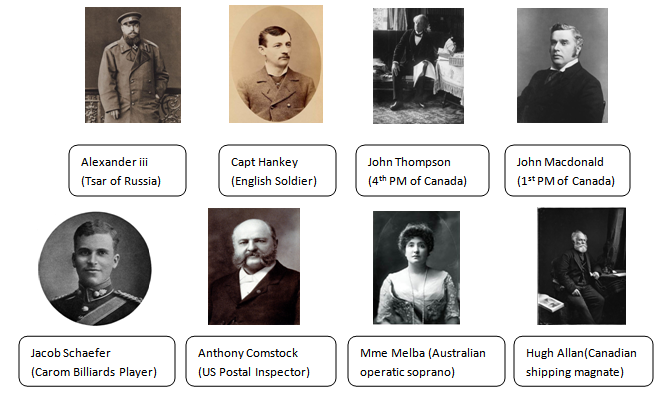
\includegraphics[scale=0.79]{ip}
\caption{Some of the top 30 influential persons obtained from the dataset and also found on Wikipedia during evaluation}
\label{figure:inf}
\vspace*{-10pt}

\end{center}
\end{figure*}

%%%%%%%%%%%%%%%%%%%%%%%%%%DOUBT HERE : This has been mentioned again in the discussion section.
%Most of the false positives, although influential in other respects, were not  influential \emph{person} entities. This can be attributed to the incorrect PNER (Person Named Entity Recognition) on noisy OCR data.
%Other reasons for obtaining false positives include: less information about these entities on Wikipedia as well as named entity disambiguation problem leading to high IPI score for several different persons having same names across the corpus.
% False positives are obtained for person entities  such as ``mr got" which is not a person entity at all and for entities such as ``ann arbor" and ``van cortlandt" which are  locations but were recognized incorrectly as person entities.
